\chapter{Communication between Software and Arduino}
\thispagestyle{empty}
\label{sec:sw-env}

\newcommand{\LocSWfig}{\Origin/user-code/sw-env/figures}
\newcommand{\LocSWscicode}{\Origin/user-code/sw-env/scilab}
\newcommand{\LocSWscibrief}[1]{{\texttt
                  Origin/user-code/sw-env/scilab/#1}, see \fnrefp{fn:file-loc}}
\newcommand{\LocSWardcode}{\Origin/user-code/sw-env/arduino}
\newcommand{\LocSWardbrief}[1]{{\tt \seqsplit{
                        Origin/user-code/sw-env/arduino/#1}}, see \fnrefp{fn:file-loc}}

\newcommand{\LocSWchkcode}{\Origin/tools/scilab}
\newcommand{\LocSWchkbrief}[1]{{\tt \seqsplit{
                        Origin/tools/scilab/#1}}, see \fnrefp{fn:file-loc}}
\newcommand{\LocSWfirmcode}{\Origin/tools/floss-firmware}
\newcommand{\LocSWfirmbrief}[1]{{\tt \seqsplit{
                        Origin/tools/floss-firmware/#1}}, see \fnrefp{fn:file-loc}}

\newcommand{\LocFIMpycode}{\Origin/tools/python}  %added for python
\newcommand{\LocFIMpybrief}[1]{{\tt \seqsplit{%
                        Origin/tools/python/#1}}, see \fnrefp{fn:file-loc}} % added for python


\newcommand{\LocFIMjuliacode}{\Origin/tools/julia}  %added for julia
\newcommand{\LocFIMjuliabrief}[1]{{\tt \seqsplit{%
                        Origin/tools/julia/#1}}, see \fnrefp{fn:file-loc}} % added for julia

%%%%%%OpenModelica Starts
\newcommand{\LocFIMOpenModelicacode}{\Origin/tools/openmodelica/windows/}  %added for OpenModelica
\newcommand{\LocFIMOpenModelicabrief}[1]{{\tt \seqsplit{%
                        Origin/tools/openmodelica/windows/#1}}, see \fnrefp{fn:file-loc}} % added for OpenModelica

%%%%%OpenModelica Ends


In this chapter, we shall briefly walk through the software
environment that needs to be set up before we could start with the
\arduino\ board-based experiments. We shall start with the \arduino\
compatible Integrated Development Environment (IDE), termed as Arduino
IDE, that would be used to load the FLOSS firmware on to the
microcontroller. The FLOSS firmware to be loaded could be developed to serve
different purposes as per the requirement. For example, 
\begin{itemize}
      \item To run \arduino\ stand-alone, without waiting for any commands
            from other software or hardware, for the specified time or until
            power off
      \item To decode the commands sent by other software, such as Scilab, Python, 
            Julia, OpenModelica, etc., through a serial port, and 
            execute the given instructions %\item Combination of the above two
\end{itemize}
Next, we shall discuss other open-source software
tools and a related toolbox that can communicate with \arduino\ 
over a serial port using RS232 protocol. 

% Subsequently, we shall discuss other open-source software tools such as Python, Julia, and OpenModelica. 

\section{Arduino IDE}\label{arduino-ide}
\label{sec:ard-start}
Arduino development environment is compatible with popular desktop
operating systems. In this section, we will learn to set up this tool
for the computers running Microsoft Windows or Linux. Later, we shall
explore the important menu options in the Arduino IDE and run a sample
program.  The following two steps have to be followed whatever operating
system is used:

\begin{enumerate}
      \item To begin, we need an \arduino\ board with a USB cable (A plug to
            B plug) as shown in \figref{arduino}.
      \item Connect it to a computer and power it up. The moment you connect \arduino\
            to the computer, an on-board power LED will turn ON.
\end{enumerate}

\subsection{Downloading and installing on Windows}
First, carry out the steps numbered 1 and 2 given above.
Starting from download, we shall go through the steps to set up
Arduino IDE on Windows OS:

\begin{enumerate}
      \setcounter{enumi}2
      \item Visit the URL, {\tt https://www.arduino.cc/en/software}. On the 
            right right side of the page, locate the link \emph{Windows ZIP file} and click on it.  
            This may redirect you to the download/donate page. Read the instructions and proceed with the
            download.
      \item Extract the downloaded ZIP file to Desktop. Do not alter any
            file or directory structure.
      \item Click on the Windows Start Menu, and open up the ``Control
            Panel''.
      \item While in the Control Panel, navigate to ``System and Security'',
            click on ``System'' and then choose the ``Device Manager''.
      \item Look for ``Other devices'' in the ``Device Manager'' list,
            expand and locate ``Unknown device''.  This may be similar to what
            is shown in \figref{win-device-manager}. In case, you don't see  
            ``Unknown device,'' look for ``Ports (COM \& LPT)'' and expand it to locate 
            ``USB Serial Device (COM2)''.
            This may be similar to what is shown in \figref{win-device-manager-com}.
      \item Right-click on the ``Unknown device'' (or ``USB Serial Device (COM2)'' as shown in 
            the previous step) and select the ``Update Driver Software'' (or ``Update driver'') option 
            as shown in \figref{win-dri-update}. 
      \item Next, choose the ``Browse my computer for Driver software''
            option.
      \item Navigate to the newly extracted Arduino folder on the Desktop and
            select ``drivers'' folder.
      \item Windows will now finish the driver installation. The Arduino IDE
            is ready for use.
\end{enumerate}
To launch Arduino IDE, browse to extracted Arduino folder on the Desktop and double click on ``arduino.exe''.
\begin{figure}
      \centering
      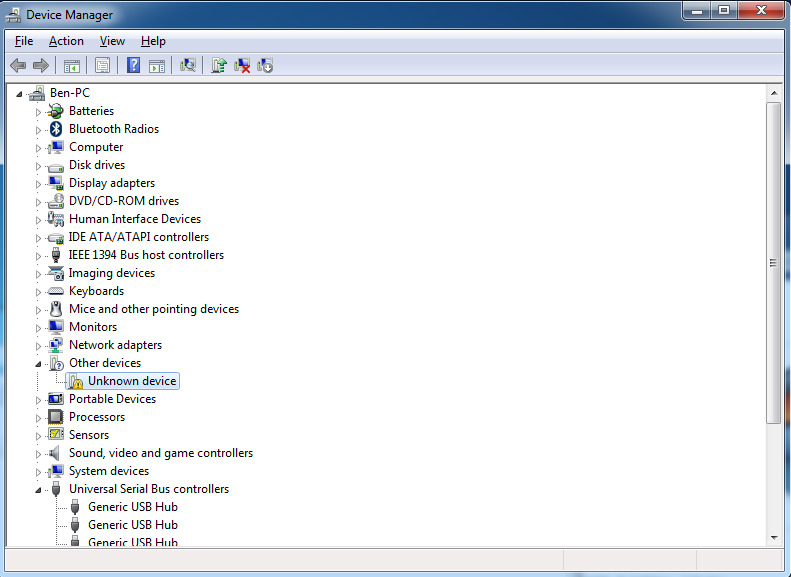
\includegraphics[width=\linewidth]{\LocHWfig/hw-device-manager.jpg}
      \caption{Windows device manager}
      \label{win-device-manager}
\end{figure}

\begin{figure}
      \centering
      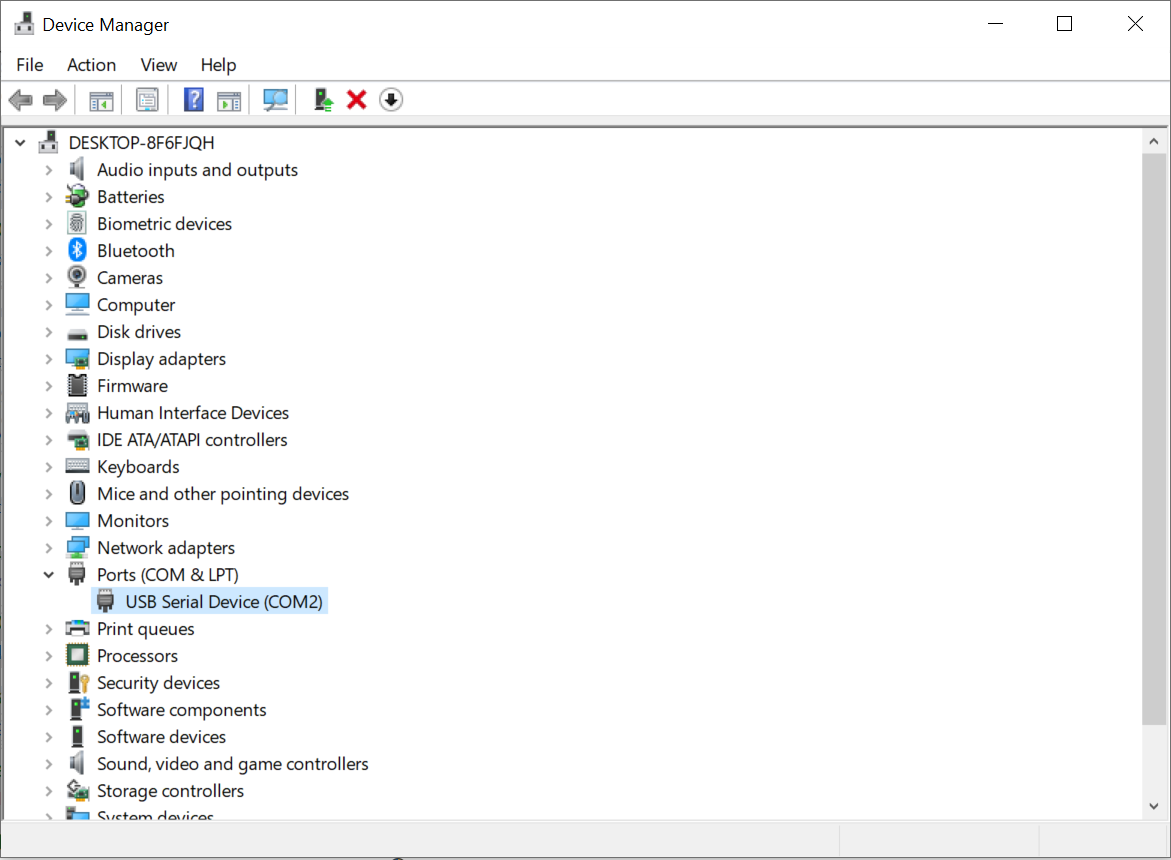
\includegraphics[width=\linewidth]{\LocSWfig/device-manager-com.png}
      \caption{Windows device manager}
      \label{win-device-manager-com}
\end{figure}

\begin{figure}
      \centering
      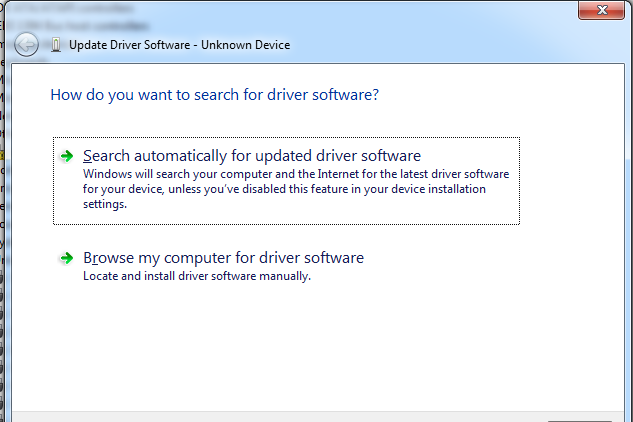
\includegraphics[width=\linewidth]{\LocHWfig/update-driver.png}
      \caption{Windows update driver option}
      \label{win-dri-update}
\end{figure}


\subsection{Downloading and installing on GNU/Linux Ubuntu}
We will now explain the installation of Arduino software on the
GNU/Linux operating system. We shall perform the installation on the 64-bit 
Ubuntu 18.04 LTS operating system.  These
instructions will work for other GNU distributions too, with little or
no modification.  First, carry out the steps numbered 1 and 2 given
above.  Then carry out the following:

\begin{enumerate}
      \setcounter{enumi}2
      \item First, update your system. Open the terminal emulator, type,
            {\tt sudo apt-get update} and press Enter. 
      \item Find out your operating system support for 64-bit
            instructions. Open the terminal emulator and type, {\tt uname -m}
      \item If it returns ``x86\_64'', then your computer has 64-bit
            operating system.   There is no visible performance difference in 32
            and 64-bit Arduino versions.
      \item Download the suitable Arduino Software version (32 or 64-bit)
            from \\ {\tt https://www.arduino.cc/en/software}.  As mentioned
            earlier, we will perform experiments with a 64-bit installation.
            
      \item At the time of writing this book, we worked with version 1.8.13.
            Assuming that you have downloaded the tar file in 
            the Downloads directory, execute the following
            commands on the terminal:
            \begin{quote}
                  {\tt cd {\large\textasciitilde}/Downloads\\
                        tar -xvf arduino-1.8.13-linux64.tar.xz\\
                        sudo mv arduino-1.8.13 /opt}
            \end{quote}
            
      \item In the same terminal session, install the required Java Runtime
            Environment with a command like,
            {\tt sudo apt-get -y install openjdk-8-jre}
            
      \item \label{itm:port-check} Execute the
            following command on the terminal to list the serial port number.\\
            {\tt ls /dev/ttyACM*}\\
            Note down the serial device filename.  Suppose that it
            is {\tt ttyACM0}.
      \item \label{itm:port-access} To make the USB port available to all users, set the read-write
            permission to the listed port:
            {\tt sudo chmod a+rw /dev/ttyACM0}. Each time you plug the \arduino\
            into the computer, you need to execute the commands given in the steps 
            numbered \ref{itm:port-check} and \ref{itm:port-access}. 
            
      % \item \label{itm:create-shortcut} Create a shortcut on the desktop:\\
      %       {\tt cd {\large \textasciitilde}/Desktop\\
      %       ln -s /opt/arduino-1.8.13/arduino}
      % \item \label{itm:give-permission} Give executable permission to this file through the following
      %       command on the terminal: {\tt chmod +x arduino}
            %   Ubuntu opens executable text files with an editor instead of
            %   executing them. To be able execute a file, open the ``Files''
            %   program from the launcher, go to menu ``Edit'', ``Preferences'', tab
            %   ``Behavior'' and set ``Executable Text Files'' to ``Ask each time'',
            %   as shown in \figref{ard-lin-executable}.
            
\end{enumerate}
% \begin{figure}
%   \centering
%   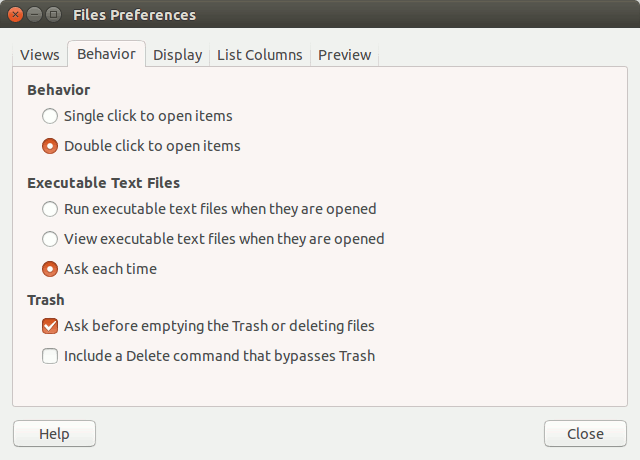
\includegraphics[scale=0.5]{\LocHWfig/executable.png}
%   \caption{Executable permission to Arduino IDE}
%   \label{ard-lin-executable}
% \end{figure}
% Then double click the Arduino shortcut on the Desktop and, click ``Run''
% in the dialog window to start the Arduino IDE. The dialog box is shown in \figref{ard-lin-run} for reference.
% \begin{figure}
%       \centering
%       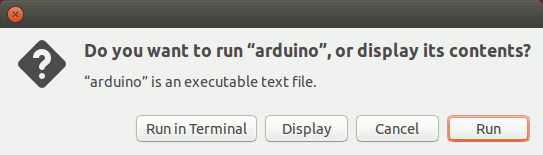
\includegraphics[scale=0.5]{\LocHWfig/run.png}
%       \caption{Confirmation for executing Arduino script}
%       \label{ard-lin-run}
% \end{figure}
The Arduino IDE is now ready for use. To launch it, carry out the steps given below:
\begin{enumerate}
      \item Open a terminal by pressing the Alt+Ctrl+T keys together.
      \item Navigate into the {\tt opt} directory, as shown in \figref{arduino-opt}.\\
      {\tt cd /opt/arduino-1.8.13/}
      \item Start the Arduino IDE by executing the command {\tt ./arduino}
\end{enumerate}


% There are chances that you might not 
% get the Arduino shortcut on your Desktop after executing the commands given in 
% steps numbered \ref{itm:create-shortcut} and \ref{itm:give-permission}. 
% In that case, you can navigate into the {\tt /opt/} directory and execute the 
% commands as given in \figref{arduino-opt} to start the Arduino IDE. 

\begin{figure}
      \centering
      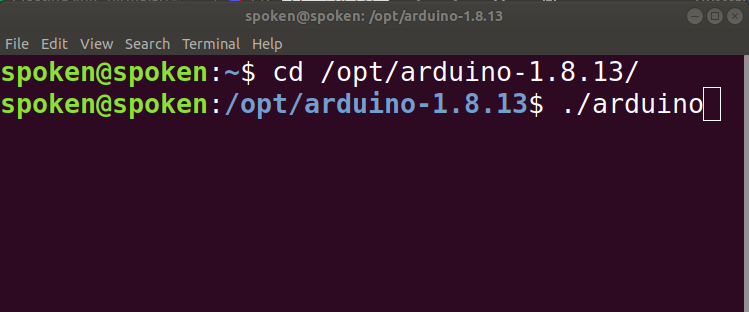
\includegraphics[width=\lgfig]{\LocSWfig/launch-arduino-opt.png}
      \caption{Linux terminal to launch Arduino IDE}
      \label{arduino-opt}
\end{figure}


\subsection{Arduino Development Environment}
\label{sec:Arduino-IDE}
The Arduino development environment, as shown in \figref{ard-ide},
consists of 
a text editor for writing code, a message area, a text console, a
toolbar with buttons for common functions, and a series of menus. It
connects to the Arduino hardware to upload programs and communicate
with them.

\begin{figure}
      \centering
      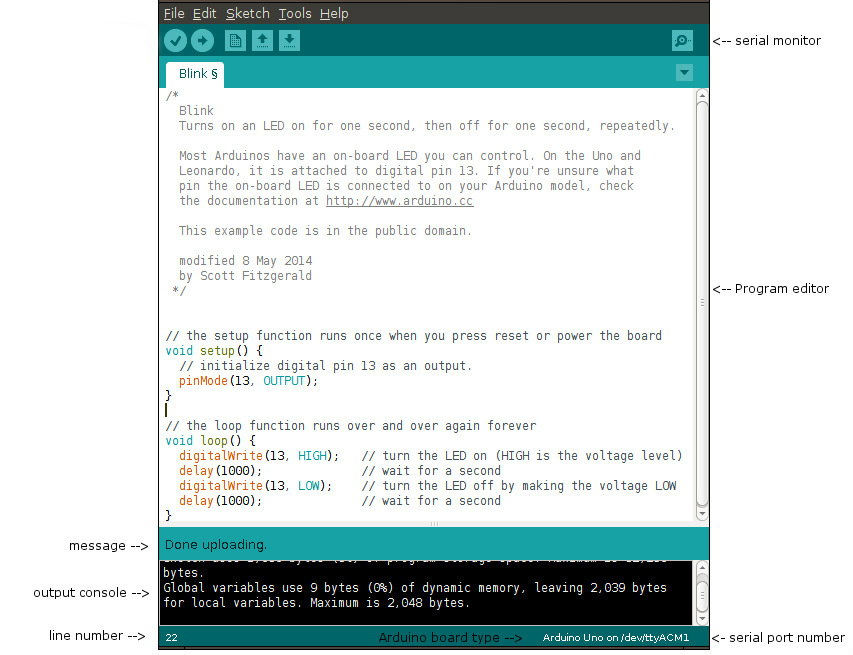
\includegraphics[width=\linewidth]{\LocHWfig/arduino-ide.jpg}
      \caption{Arduino IDE}
      \label{ard-ide}
\end{figure}
Software written using Arduino is called sketches. These sketches are
written in the text editor. Sketches are saved with the file extension
``.ino''. The frequently used icons shown in the toolbar, below the menu bar, are explained next. The names of these icons can be viewed by hovering the mouse pointer over each of them.

\begin{enumerate}
      \item Verify: Checks your code for errors
      \item Upload: Compiles your code and uploads it to the Arduino I/O
            board
      \item New: Creates a new sketch
      \item Open: Presents a menu of all the sketches in your
            sketchbook - clicking one will open it within the current window
      \item Save: Saves your sketch
      \item Serial Monitor: Opens the serial port window - the location of
            this is shown in the top right-hand corner of \figref{ard-ide}
\end{enumerate}
Note that these appear from left to right in the editor window. Next, we shall go through the additional useful options under the menu.
\begin{enumerate}
      \item File
            \begin{enumerate}
                  \item Examples: Examples that come at the time of installation
                  \item Page Setup: Configures the page parameters for the printer
                  \item Preferences: Customizes font, language, and other parameters for
                        the IDE
            \end{enumerate}
      \item Sketch
            \begin{enumerate}
                  \item Include Library: Adds a library to your sketch by inserting {\tt
                                    \#include} statements at the start of your code
            \end{enumerate}
      \item Tools
            \begin{enumerate}
                  \item Auto Format: Indents code so that opening and closing curly
                        braces line up
                  \item Archive Sketch: Archives a copy of the current sketch in .zip
                        format. The archive is placed in the same directory as the sketch.
                  \item Board: Selects the board that you're using
                  \item Port: This menu contains all the serial devices (real or
                        virtual) on your machine. It should automatically refresh every time
                        you open the top-level tools menu.
                  \item Programmer: This can be used to select a hardware programmer when programming a board or chip and not using the onboard USB-serial
                        connection. Normally you won't need this, but if you're burning a
                        bootloader to a new microcontroller, you will use this.
                  \item Burn Bootloader: The items in this menu allow you to burn a
                        bootloader onto the microcontroller on an Arduino board. This is not
                        required for normal use of an Arduino board but is useful if you
                        purchase a new ATmega microcontroller (which normally comes without a
                        bootloader). Ensure that you've selected the correct board from the
                        Boards menu before burning the bootloader.
            \end{enumerate}
\end{enumerate}

\subsection{Testing Arduino with a sample program}
\label{sec:testing-arduino}
Now, as we have a basic understanding of Arduino IDE, let us try an
example program.
\begin{enumerate}
      \item Open the Arduino IDE by clicking the shortcut ``arduino'' from
            Desktop in Ubuntu. In MS Windows browse to extracted Arduino folder
            on Desktop and double click on ``arduino.exe''.
      \item In the Arduino IDE, to know the path of your sketch files,
            navigate to File, then Preferences and then locate the ``Sketchbook
            location'' text box at the top.  You may change the path of your
            storage location. In this book, we will keep it unchanged. The path
            will be different for Windows and Ubuntu.
      \item To load a sample program, navigate and click on sketch ``File'',
            then Examples, then 01.Basics, and then Blink.
      \item A new IDE instance will open with Blink LED code.  You may close
            the previous IDE window now.
      \item Click ``verify'' to compile. The ``status bar'' below the text editor
            shall show ``Done compiling'' on success.
      \item Connect \arduino\ board to PC. You may connect the board
            before writing the sketch too.
      \item Now, navigate to ``Tools'', then Port, and select the available
            port. If the port option is greyed out (or disabled) then reinsert the
            USB cable to the PC.
      \item Now select the upload button to compile and send the firmware to
            the Arduino Uno board.
      \item If the upload is successful, you will notice the onboard orange LED
            next to the Arduino logo will start blinking.
      \item It is safe to detach the USB cable at any moment.
\end{enumerate}

Arduino programming syntax is different from other languages. In an
embedded setup, a program is expected to run forever. To facilitate
this, the Arduino programming structure has two main functions: {\tt setup()}:
Used to initialize variables, pin modes, libraries, etc. The setup
function will run only once after each powerup or board reset.
{\tt loop()}: Code inside this function runs forever. An Arduino program
must have {\tt setup()} and {\tt loop()} functions.  We will give several examples
in this book to explain this usage.

An inbuilt offline help is available within the IDE. You may access
the explanation on IDE by navigating to ``Help'' and then
Environment.

\subsection{FLOSS Firmware}
We have provided a code to check whether the FLOSS firmware has been
properly installed.  The first few lines of this code follow. 

\begin{ardcode}
      \acaption{First 10 lines of the FLOSS firmware}{First 10 lines of
            the FLOSS firmware.  Available at
            \LocSWfirmbrief{floss-firmware.ino}. Following the
            steps given in sections \ref{sec:Arduino-IDE} and 
            \ref{sec:testing-arduino}, open this code in 
            Arduino IDE and upload it to \arduino. 
            Once the upload is successful, you should expect a success message 
            at the bottom of Arduino IDE, as shown in \figref{ard-ide}. }
      \label{ard:firmware}
      \lstinputlisting[firstline=1,lastline=10]
      {\LocSWfirmcode/floss-firmware.ino}
\end{ardcode}

% \subsection{Arduino firmware to work with scilab toolbox}
% \label{sec:firmware}
% A firmware is basically a program that continuously runs inside a
% microcontroller. It is a collection of routines corresponding to the
% required functionalities. It is typically written in Assembly and C
% programming language. It is compiled and converted into
% binary(hexadecimal values with addresses) for the target
% microcontroller. The binary file(also called hex file) is then
% uploaded to the microcontroller’s internal ROM. The firmware that has to
% be used to work with scilab toolbox is at \ardref{ard:firmware}.  It
% is an Arduino IDE compatible file and can be opened in an Arduino
% IDE. Let us see a brief explanation of this firmware.

% The firmware used for Arduino Uno in this book has the following tasks
% to perform:
% \begin{enumerate}
% \item Reading instructions from a computer(running Scilab) over serial
%   interface and decoding them. 
% \item Performing the task mentioned in the instruction.
% \item Optionally sending data back to the computer over an serial
%   interface.
% \end{enumerate}
% Let us see a simple example of reading values from the LDR that is
% on the shield.

% The firmware waits for a particular character (command) to be sent
% from the computer. The character “A”, in quoted form, as shown here,
% is reserved for analog read
% routine. So if Scilab wants analog values from the microcontroller, it
% sends the character “A” to Arduino Uno. On receiving “A”, the Arduino
% Uno 
% jumps to the routine of Analog read. Here it again waits for the
% computer to now send the pin number from where it is supposed to read
% the LDR value. This pin number is in ASCII text. Arduino Uno first
% checks if the ASCII lies between a valid range. If yes, it takes its
% ASCII value as a valid pin number. The value 48 is subtracted from it
% to reveal the character and thus the pin number. This pin number is
% then sent to the analogRead() function. The analogRead() function is
% an inbuilt Arduino function imported from the header file. The
% analogRead() function then actually reads from the pin and returns the
% analog value. This value is then sent back to the
% computer(Scilab). The correct firmware must be loaded inside Arduino
% Uno to be able to successfully carry out any of the experiment
% explained throughout this book. It is strongly recommended to confirm
% this before proceeding. 